\documentclass[12pt,a4paper]{article}
\usepackage[utf8]{inputenc}
\usepackage{amsmath}
\usepackage{amsfonts}
\usepackage{amssymb}
\usepackage{graphicx}
\usepackage[]{xspace}
\usepackage{tikz} %for diagrams
\usetikzlibrary{calc,math,arrows}
\begin{document}
\begin{figure}
	\centering
	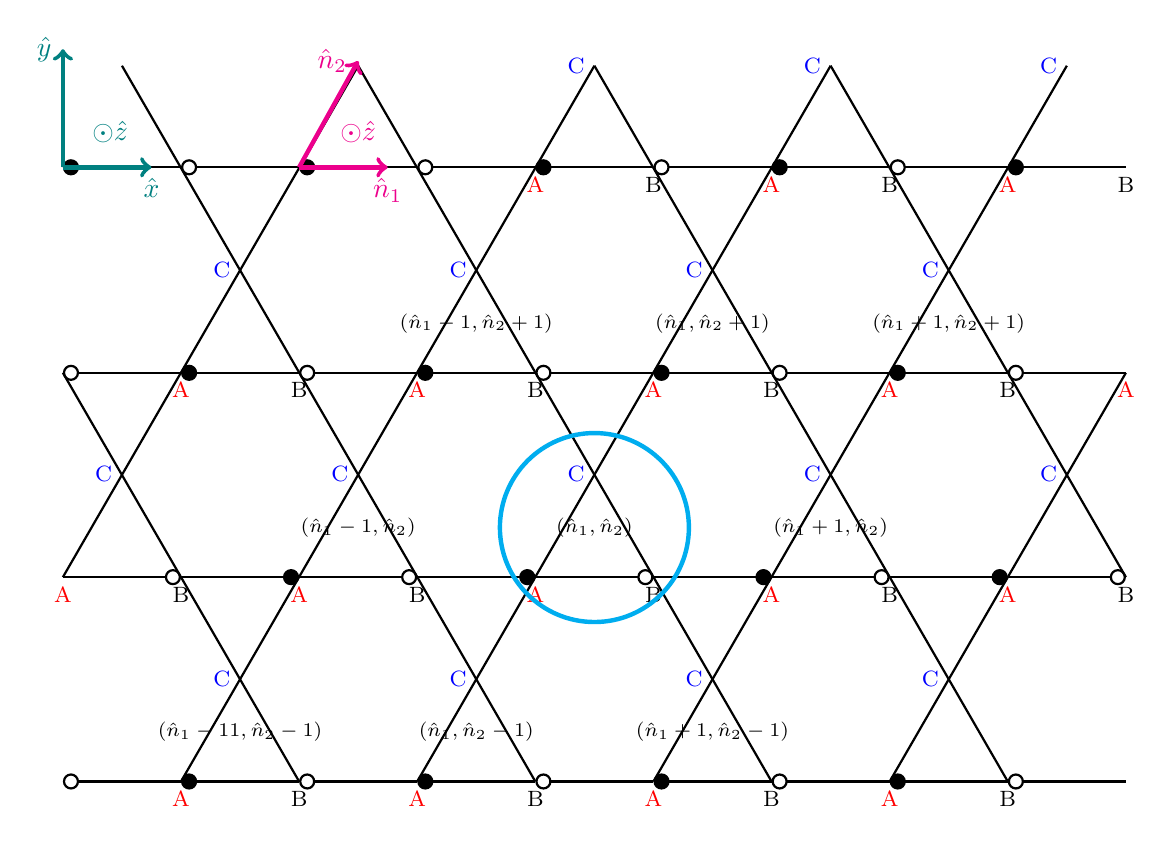
\begin{tikzpicture}[scale = 1.5] %change the scale to fit in your slide
			\foreach \x in {0,2,...,8}
				{\draw[thick, o-] (\x,0)--(\x+1,0);
				\draw[thick,-o] (\x,1.73)--(\x+1,1.73);
				\node[below,red] at (\x,1.73) {{\footnotesize A}};
				\node[below] at (\x+1,1.73) {{\footnotesize B}};
				\node[left,blue] at (\x+0.5,2.6) {{\footnotesize C}};
				\draw[thick, o-] (\x,3.46)--(\x+1,3.46);
				\node[below,red] at (\x+1,3.46) {{\footnotesize A}};
				\draw[thick, *-] (\x,5.2)--(\x+1,5.2);};		
			\foreach \x in {1,3,5,7} 
				{\node[below,red] at (\x,0) {{\footnotesize A}};
				 \draw[thick,*-] (\x,0)--(\x+1,0);
				 \node[below] at (\x+1,0) {{\footnotesize B}};
				 \node[left,blue] at (\x+0.5,0.87) {{\footnotesize C}};
				 \draw[thick,-*] (\x,1.73)--(\x+1,1.73);
				 \draw[thick,*-] (\x,3.46)--(\x+1,3.46);
				 \node[below] at (\x+1,3.46) {{\footnotesize B}};
				 \node[left,blue] at (\x+0.5,4.33) {{\footnotesize C}};
				 \draw[thick,o-] (\x,5.2)--(\x+1,5.2);};
			\foreach \x in {1,3,5}
				{\draw[thick] (\x,0) -- (\x+3.5,6.06);};
			\draw[thick] (7,0) -- (9,3.46);
			\draw[thick] (2,0) -- (0,3.46);
			\draw[thick] (0,1.73)--(2.5,6.06);
			\draw[thick] (9,1.73)--(6.5,6.06);
			\foreach \x in {4,6,8}
				{\draw[thick] (\x,0) -- (\x-3.5,6.06);
				\node[below,red] at (\x,5.2) {{\footnotesize A}};
				\node[below] at (\x+1,5.2) {{\footnotesize B}};
				\node[left,blue] at (\x+0.5,6.06) {{\footnotesize C}};};	
			\draw[ultra thick,teal,->] (0,5.2)--(0.75,5.2) node[below]{$\hat{x}$};
			\draw[ultra thick,teal,->] (0,5.2)--(0,6.2) node[left]{$\hat{y}$};
			\node[teal] at (0.4,5.5) {$\odot \hat{z}$};
			\draw[ultra thick,magenta,->] (2,5.2)--(2.75,5.2) node[below]{$\hat{n}_1$};
			\draw[ultra thick,magenta,->] (2,5.2)--(2.5,6.1) node[left]{$\hat{n}_2$};
			\node[magenta] at (2.5,5.5) {$\odot \hat{z}$};
			\draw [cyan, ultra thick] (4.5,2.15) circle [radius=.8];
			\node at (4.5,2.15) {{\scriptsize $(\hat{n}_1,\hat{n}_2)$}};
			\node at (6.5,2.15) {{\scriptsize $(\hat{n}_1+1,\hat{n}_2)$}};
			\node at (2.5,2.15) {{\scriptsize $(\hat{n}_1-1,\hat{n}_2)$}};
			\node at (3.5,3.88) {{\scriptsize $(\hat{n}_1-1,\hat{n}_2+1)$}};
			\node at (5.5,3.88) {{\scriptsize $(\hat{n}_1,\hat{n}_2+1)$}};
			\node at (7.5,3.88) {{\scriptsize $(\hat{n}_1+1,\hat{n}_2+1)$}};
			\node at (5.5,0.42) {{\scriptsize $(\hat{n}_1+1,\hat{n}_2-1)$}};
			\node at (3.5,0.42) {{\scriptsize $(\hat{n}_1,\hat{n}_2-1)$}};
			\node at (1.5,0.42) {{\scriptsize $(\hat{n}_1-11,\hat{n}_2-1)$}};
	\end{tikzpicture}
    \caption{Kagome}
    \label{fig:fireball}
\end{figure}
\end{document}